
%======================================================================
%   D O C U M E N T   P R E A M B L E
% Specify the document class, default style attributes, and page dimensions, etc.
% For hyperlinked PDF, suitable for viewing on a computer, use this:
\documentclass[letterpaper,12pt,titlepage,oneside,final]{book}
 
% For PDF, suitable for double-sided printing, change the PrintVersion variable below to "true" and use this \documentclass line instead of the one above:
%\documentclass[letterpaper,12pt,titlepage,openright,twoside,final]{book}

% Some LaTeX commands I define for my own nomenclature.
% If you have to, it's easier to make changes to nomenclature once here than in a million places throughout your thesis!
\newcommand{\package}[1]{\textbf{#1}} % package names in bold text
\newcommand{\cmmd}[1]{\textbackslash\texttt{#1}} % command name in tt font 
\newcommand{\href}[1]{#1} % does nothing, but defines the command so the print-optimized version will ignore \href tags (redefined by hyperref pkg).
%\newcommand{\texorpdfstring}[2]{#1} % does nothing, but defines the command
% Anything defined here may be redefined by packages added below...

% This package allows if-then-else control structures.
\usepackage{ifthen}
\newboolean{PrintVersion}
\setboolean{PrintVersion}{false}
% CHANGE THIS VALUE TO "true" as necessary, to improve printed results for hard copies by overriding some options of the hyperref package, called below.

%\usepackage{nomencl} % For a nomenclature (optional; available from ctan.org)
\usepackage{amsmath,amssymb,amstext} % Lots of math symbols and environments
\usepackage{graphicx} % For including graphics N.B. pdftex graphics driver 
\usepackage{subcaption}
\usepackage{enumitem}
\usepackage{booktabs}
\usepackage{siunitx}
% Hyperlinks make it very easy to navigate an electronic document.
% In addition, this is where you should specify the thesis title and author as they appear in the properties of the PDF document.
% Use the "hyperref" package 
% N.B. HYPERREF MUST BE THE LAST PACKAGE LOADED; ADD ADDITIONAL PKGS ABOVE
\usepackage[pagebackref=false]{hyperref} % with basic options
%\usepackage[pdftex,pagebackref=true]{hyperref}
		% N.B. pagebackref=true provides links back from the References to the body text. This can cause trouble for printing.
\usepackage{cleveref}
\hypersetup{
    plainpages=false,       % needed if Roman numbers in frontpages
    unicode=false,          % non-Latin characters in Acrobat’s bookmarks
    pdftoolbar=true,        % show Acrobat’s toolbar?
    pdfmenubar=true,        % show Acrobat’s menu?
    pdffitwindow=false,     % window fit to page when opened
    pdfstartview={FitH},    % fits the width of the page to the window
%    pdftitle={uWaterloo\ LaTeX\ Thesis\ Template},    % title: CHANGE THIS TEXT!
%    pdfauthor={Author},    % author: CHANGE THIS TEXT! and uncomment this line
%    pdfsubject={Subject},  % subject: CHANGE THIS TEXT! and uncomment this line
%    pdfkeywords={keyword1} {key2} {key3}, % list of keywords, and uncomment this line if desired
    pdfnewwindow=true,      % links in new window
    colorlinks=true,        % false: boxed links; true: colored links
    linkcolor=black,         % color of internal links
    citecolor=black,        % color of links to bibliography
    filecolor=magenta,      % color of file links
    urlcolor=cyan           % color of external links
}
\ifthenelse{\boolean{PrintVersion}}{   % for improved print quality, change some hyperref options
\hypersetup{	% override some previously defined hyperref options
%    colorlinks,%
    citecolor=black,%
    filecolor=black,%
    linkcolor=black,%
    urlcolor=black}
}{} % end of ifthenelse (no else)

\usepackage[automake,toc,abbreviations]{glossaries-extra} % Exception to the rule of hyperref being the last add-on package
% If glossaries-extra is not in your LaTeX distribution, get it from CTAN (http://ctan.org/pkg/glossaries-extra), 
% although it's supposed to be in both the TeX Live and MikTeX distributions. There are also documentation and 
% installation instructions there.

% Setting up the page margins...
% uWaterloo thesis requirements specify a minimum of 1 inch (72pt) margin at the
% top, bottom, and outside page edges and a 1.125 in. (81pt) gutter margin (on binding side). 
% While this is not an issue for electronic viewing, a PDF may be printed, and so we have the same page layout for both printed and electronic versions, we leave the gutter margin in.
% Set margins to minimum permitted by uWaterloo thesis regulations:
% \setlength{\marginparwidth}{0pt} % width of margin notes
% N.B. If margin notes are used, you must adjust \textwidth, \marginparwidth
% and \marginparsep so that the space left between the margin notes and page
% edge is less than 15 mm (0.6 in.)
% \setlength{\marginparsep}{0pt} % width of space between body text and margin notes
% \setlength{\evensidemargin}{0.125in} % Adds 1/8 in. to binding side of all 
% even-numbered pages when the "twoside" printing option is selected
% \setlength{\oddsidemargin}{0.125in} % Adds 1/8 in. to the left of all pages when "oneside" printing is selected, and to the left of all odd-numbered pages when "twoside" printing is selected
% \setlength{\textwidth}{6.375in} % assuming US letter paper (8.5 in. x 11 in.) and side margins as above

\usepackage{titlesec}
\usepackage{ragged2e}

\titleformat{\chapter}[block]
  {\normalfont\normalsize\bfseries\Centering\hyphenpenalty=10000\exhyphenpenalty=10000\parindent=0pt}
  {CHAPTER \thechapter:}{0.5em}
  {\MakeUppercase}

\titleformat{name=\chapter,numberless}[block]
  {\normalfont\normalsize\bfseries\Centering\parindent=0pt}
  {}{0pt}
  {\MakeUppercase}

\titlespacing*{\chapter}{0pt}{0pt}{24pt}

\titleformat{\section}
  {\normalfont\normalsize\bfseries}
  {\thesection}
  {1em}
  {}

\titlespacing*{\section}{0pt}{18pt}{6pt}

\titleformat{\subsection}
  {\normalfont\normalsize\bfseries}
  {\thesubsection}
  {1em}
  {}

\titlespacing*{\subsection}{0pt}{14pt}{6pt}  % space after

% --- Native LaTeX Margins for Troy University (US Letter: 8.5 x 11 in) ---

% Horizontal Margins (Target: Left = 1.5 in, Right = 1.0 in)
% LaTeX adds 1.0 in by default, so offset = Target - 1.0 in
\setlength{\oddsidemargin}{0.5in}    % 1.0 in default + 0.5 in = 1.5 in left margin
\setlength{\evensidemargin}{0.5in}   % 1.5 in left margin if twoside is used
\setlength{\textwidth}{6.0in}        % 8.5 in paper width - 1.5 in left - 1.0 in right = 6.0 in

% Vertical Margins (Target: Top = 1.0 in, Bottom = 1.0 in)
\setlength{\topmargin}{0.0in}        % 1.0 in default + 0.0 in = 1.0 in to top of header
\setlength{\headheight}{0.0in}       % No header text
\setlength{\headsep}{0.0in}          % No header separation
\setlength{\textheight}{9.0in}       % 11.0 in paper height - 1.0 in top - 1.0 in bottom = 9.0 in

% Page Number Placement (Target: Centered, 0.5 in from bottom edge of sheet)
% Distance from bottom of text body (which is 1.0 in above sheet edge) to page number:
\setlength{\footskip}{0.5in}         % 1.0 in margin - 0.5 in = 0.5 in above sheet bottom

% Margin notes / side notes disabled
\setlength{\marginparwidth}{0pt}
\setlength{\marginparsep}{0pt}
\raggedbottom

% The following statement specifies the amount of space between paragraphs. Other reasonable specifications are \bigskipamount and \smallskipamount.
\setlength{\parskip}{\medskipamount}

% The following statement controls the line spacing.  
% The default spacing corresponds to good typographic conventions and only slight changes (e.g., perhaps "1.2"), if any, should be made.
\renewcommand{\baselinestretch}{1} % this is the default line space setting

% By default, each chapter will start on a recto (right-hand side) page.
% We also force each section of the front pages to start on a recto page by inserting \cleardoublepage commands.
% In many cases, this will require that the verso (left-hand) page be blank, and while it should be counted, a page number should not be printed.
% The following statements ensure a page number is not printed on an otherwise blank verso page.
\let\origdoublepage\cleardoublepage
\newcommand{\clearemptydoublepage}{%
  \clearpage{\pagestyle{empty}\origdoublepage}}
\let\cleardoublepage\clearemptydoublepage

% Define Glossary terms (This is properly done here, in the preamble and could also be \input{} from a separate file...)
% Main glossary entries -- definitions of relevant terminology
\newglossaryentry{computer}
{
name=computer,
description={A programmable machine that receives input data,
               stores and manipulates the data, and provides
               formatted output}
}

% Nomenclature glossary entries -- New definitions, or unusual terminology
\newglossary*{nomenclature}{Nomenclature}
\newglossaryentry{dingledorf}
{
type=nomenclature,
name=dingledorf,
description={A person of supposed average intelligence who makes incredibly brainless misjudgments}
}

% List of Abbreviations (abbreviations type is built in to the glossaries-extra package)
\newabbreviation{aaaaz}{AAAAZ}{American Association of Amateur Astronomers and Zoologists}

% List of Symbols
\newglossary*{symbols}{List of Symbols}
\newglossaryentry{rvec}
{
name={$\mathbf{v}$},
sort={label},
type=symbols,
description={Random vector: a location in n-dimensional Cartesian space, where each dimensional component is determined by a random process}
}
\makeglossaries

%======================================================================
%   L O G I C A L    D O C U M E N T
% The logical document contains the main content of your thesis.
% Being a large document, it is a good idea to divide your thesis into several files, each one containing one chapter or other significant chunk of content, so you can easily shuffle things around later if desired.
%======================================================================
\begin{document}

%----------------------------------------------------------------------
% FRONT MATERIAL
% title page, examining committee membership (for PhD Thesis only), declaration, borrowers' page, abstract, acknowledgements,
% dedication, table of contents, list of tables, list of figures, nomenclature, etc.
%----------------------------------------------------------------------
% ============================================================
% T I T L E   P A G E
% ============================================================
% Troy University Thesis Guidelines
% Title page is counted but not numbered.
% No headers or footers on the title page.

\pagestyle{empty}
\pagenumbering{roman}

% ---------- Thesis Metadata ----------
\newcommand{\thesistitle}{Thesis Title}
\newcommand{\authorname}{KISHAN RAJDEV}

\newcommand{\thesisdegree}{Master of Science}
\newcommand{\program}{Computer Science}
\newcommand{\gradmonth}{DECEMBER}
\newcommand{\gradyear}{2026}
\newcommand{\campusname}{Troy}
\newcommand{\studentid}{1709777}
\newcommand{\advisorname}{Dr. Hyung Jae Chang}
\newcommand{\deanname}{Dr. Govind Menon}
\newcommand{\gradschooldean}{Dr. Mary Anne Templeton}
\renewcommand{\baselinestretch}{1}\normalsize

% ============================================================
% T I T L E   P A G E
% ============================================================

\begin{titlepage}
    \thispagestyle{empty}

    \begin{center}

        % Title
        \vspace*{1.0cm}

        \Large
        \textbf{\thesistitle}

        % "by"
        \vspace{1.5cm}

        \normalsize
        by

        % Author
        \vspace{0.75cm}

        \large
        \textbf{\authorname}

        % A THESIS
        \vspace{2.5cm}

        \normalsize
        \textbf{A THESIS}

        % Degree information
        \vspace{2.5cm}

        Submitted in partial fulfillment of the requirements\\
        for the degree of \thesisdegree\\
        in \program\\
        in the Graduate School of\\
        Troy University

        % Location and date
        \vspace{2.5cm}

        TROY, ALABAMA
      
        \vspace{0.25cm}
      
        \gradmonth, \gradyear

    \end{center}

\end{titlepage}


% ============================================================
% R E S T   O F   F R O N T   M A T T E R
% ============================================================
% Preliminary pages use lowercase Roman numerals.
% The title page is counted as page i but its number is suppressed.
% The acceptance page and abstract are also counted but not numbered.

\pagestyle{plain}
\setcounter{page}{2}

\cleardoublepage
\phantomsection


% ============================================================
% A C C E P T A N C E   P A G E
% ============================================================

\clearpage
\thispagestyle{empty}

\begin{center}

    % Thesis title
    \textbf{\thesistitle}

    \vspace{1.5cm}

    % Submission statement
    Submitted by Kishan Rajdev in partial fulfillment of the requirements\\
    for the degree of \thesisdegree\\
    in \program\\
    in the Graduate School of\\
    Troy University

    \vspace{1.5cm}

    Accepted on behalf of the Faculty of the Graduate School by the thesis committee:

\end{center}

% ---------- Thesis Chair ----------

\vspace{0.8cm}

\noindent
\begin{tabular*}{\textwidth}{@{\extracolsep{\fill}}p{3in}p{1.5in}@{}}
\hrulefill & \hrulefill \\
Dr. Hyung Jae Chang, Ph.D. & Date \\
Associate Professor, Computer Science & \\
Chair & \\
\end{tabular*}


% ---------- Committee Member 1 ----------

\vspace{0.8cm}

\noindent
\begin{tabular}{@{}p{3in}@{}}
\hrulefill \\
Dr. Long Ma, Ph.D. \\
Associate Professor, Computer Science
\end{tabular}


% ---------- Committee Member 2 ----------

\vspace{0.8cm}

\noindent
\begin{tabular}{@{}p{3in}@{}}
\hrulefill \\
Dr. Byungkwan Jung, Ph.D. \\
Assistant Professor, Computer Science
\end{tabular}


% ---------- Department Chair ----------

\vspace{0.8cm}

\noindent
\begin{tabular}{@{}p{3in}@{}}
\hrulefill \\
Dr. Bernard Chen, Ph.D. \\
Chair, Department of Computer Science
\end{tabular}


% ---------- Dean of the College of Arts and Sciences ----------

\vspace{0.8cm}

\noindent
\begin{tabular*}{\textwidth}{@{\extracolsep{\fill}}p{3in}p{1.5in}@{}}
\hrulefill & \hrulefill \\
Dr. Govind Menon, Ph.D. & Date \\
Dean of the College of Arts and Sciences & \\
\end{tabular*}


\cleardoublepage
\phantomsection


% ============================================================
% A B S T R A C T
% ============================================================

\addcontentsline{toc}{chapter}{Abstract}

\renewcommand{\baselinestretch}{1.5}\normalsize

\begin{center}
    \textbf{Abstract}
\end{center}

\begin{center}
    \textbf{\thesistitle}
    
    \textbf{\authorname}
\end{center}

% IMPORTANT:
% Troy requires the abstract to be one single paragraph,
% double-spaced, without indentation, and no more than 250 words.

\noindent
Deep neural networks (DNNs)....


\cleardoublepage
\phantomsection

\renewcommand{\baselinestretch}{1}\normalsize
% ============================================================
% H U M A N   O R   A N I M A L   S U B J E C T S   R E V I E W
% ============================================================

\clearpage

\addcontentsline{toc}{chapter}{Human or Animal Subjects Review Form}

\begin{center}
    \textbf{HUMAN OR ANIMAL SUBJECTS REVIEW FORM}
\end{center}

\vspace{0.5cm}

\begin{center}
    for\\[0.3cm]
    \authorname
\end{center}

\vspace{0.5cm}

\begin{center}
    \textbf{\thesistitle}
\end{center}

\vspace{1.2cm}

\noindent
This research project has been reviewed by the Institutional Review Board and approved as follows (the appropriate block must be checked by either the Thesis chair or the Chair of the Institutional Review Board):

\vspace{0.4cm}

\begin{itemize}
    \item[$\square$]
    Neither humans nor animals will be used, and this research is certified exempt from Institutional Review Board review by the thesis committee chair.

    \item[$\square$]
    Human participants will be used, and this research is certified exempt from Institutional Review Board review by the Chair of the Institutional Review Board.

    \item[$\square$]
    Human participants will be used, and this research was reviewed and is approved by the Institutional Review Board.

    \item[$\square$]
    Animal participants will be used, and this research was reviewed and is approved by the Animal Research Review Board.
\end{itemize}

\vspace{1.2cm}

\noindent
\rule{2.5in}{0.4pt}
\hfill
\rule{1.5in}{0.4pt}
\\
Signature of Thesis Committee Chair
\hfill
Date

\vspace{1.2cm}

\noindent
\rule{3.2in}{0.4pt}
\hfill
\rule{1.5in}{0.4pt}
\\
Signature of Chair of Institutional Review Board
\hfill
Date


\cleardoublepage
\phantomsection


% ============================================================
% T A B L E   O F   C O N T E N T S
% ============================================================

\renewcommand{\contentsname}{Table of Contents}
\tableofcontents

\cleardoublepage
\phantomsection


% ============================================================
% L I S T   O F   F I G U R E S
% ============================================================

\addcontentsline{toc}{chapter}{List of Figures}
\listoffigures

\cleardoublepage
\phantomsection


% ============================================================
% L I S T   O F   T A B L E S
% ============================================================

\addcontentsline{toc}{chapter}{List of Tables}
\listoftables

\cleardoublepage
\phantomsection


% ============================================================
% M A I N   T E X T
% ============================================================

% Change page numbering back to Arabic numerals.
% Chapter 1 should begin on page 1.

\pagenumbering{arabic}
\setcounter{page}{1} 

%----------------------------------------------------------------------
% MAIN BODY
% We suggest using a separate file for each chapter of your thesis.
% Start each chapter file with the \chapter command.
% Only use \documentclass or \begin{document} and \end{document} commands in this master document.
% Tip: Putting each sentence on a new line is a way to simplify later editing.
%----------------------------------------------------------------------
\renewcommand{\baselinestretch}{2}
%======================================================================
\chapter{Introduction}
%======================================================================

\section{Motivation}

Deep neural networks (DNNs) have become central to modern artificial intelligence, achieving state-of-the-art performance across a wide range of applications.... \cite{goodfellow2016deep, bishop2006pattern}.

\section{Overview}

This work investigates the relationship between computational efficiency, model diversity, and predictive reliability....


%% ============================================================
%% Chapter 2 – Background
%% Thesis: Diversity and Efficiency in Ensemble-Based
%% Uncertainty Estimation for Deep Learning
%% ============================================================

\chapter{Background}
\label{chap:background}

\section{Neural Network Classification}
\label{sec:nn_classification}
 
In a classification task defined by a dataset $\mathcal{D} = \{(\mathbf{x}_i, y_i)\}_{i=1}^{N}$, where $\mathbf{x}_i \in \mathbb{R}^d$ denotes an input feature vector and $y_i \in \{1, \ldots, K\}$ is the corresponding class label, a deep neural network defines a parametric function $f_\theta : \mathbb{R}^d \rightarrow \mathbb{R}^K$ with learnable parameters $\theta$, which maps each input to a vector of logits $\mathbf{z} = f_\theta(\mathbf{x}) \in \mathbb{R}^K$.

Class probabilities are obtained by applying the softmax function to the logits:
\begin{equation}
    p_\theta(y = k \mid \mathbf{x})
    = \frac{\exp(z_k)}{\sum_{j=1}^{K} \exp(z_j)},
    \qquad k = 1, \ldots, K
    \label{eq:softmax}
\end{equation}


\chapter{Methodology and Results}

\section{Problem Formulation}

Convolutional Neural Networks (CNNs) are widely used....

\section{Results and Discussion}

\subsection{Result table}
  
Table \ref{tab:results} reports....

\begin{table}[!h]
\centering
\caption{Results table}
\label{tab:results}
\small
\begin{tabular}{l S S S S}
\toprule
\textbf{Model} & {\textbf{ACC$\uparrow$}} & {\textbf{NLL$\downarrow$}} & {\textbf{Brier$\downarrow$}} & {\textbf{ECE$\downarrow$}} \\
\midrule
Single               & 0.913 & 0.385 & 0.140 & 0.058 \\
\bottomrule
\end{tabular}
\end{table}


\subsection{Result Figure}


\begin{figure}[!h]
  \centering
  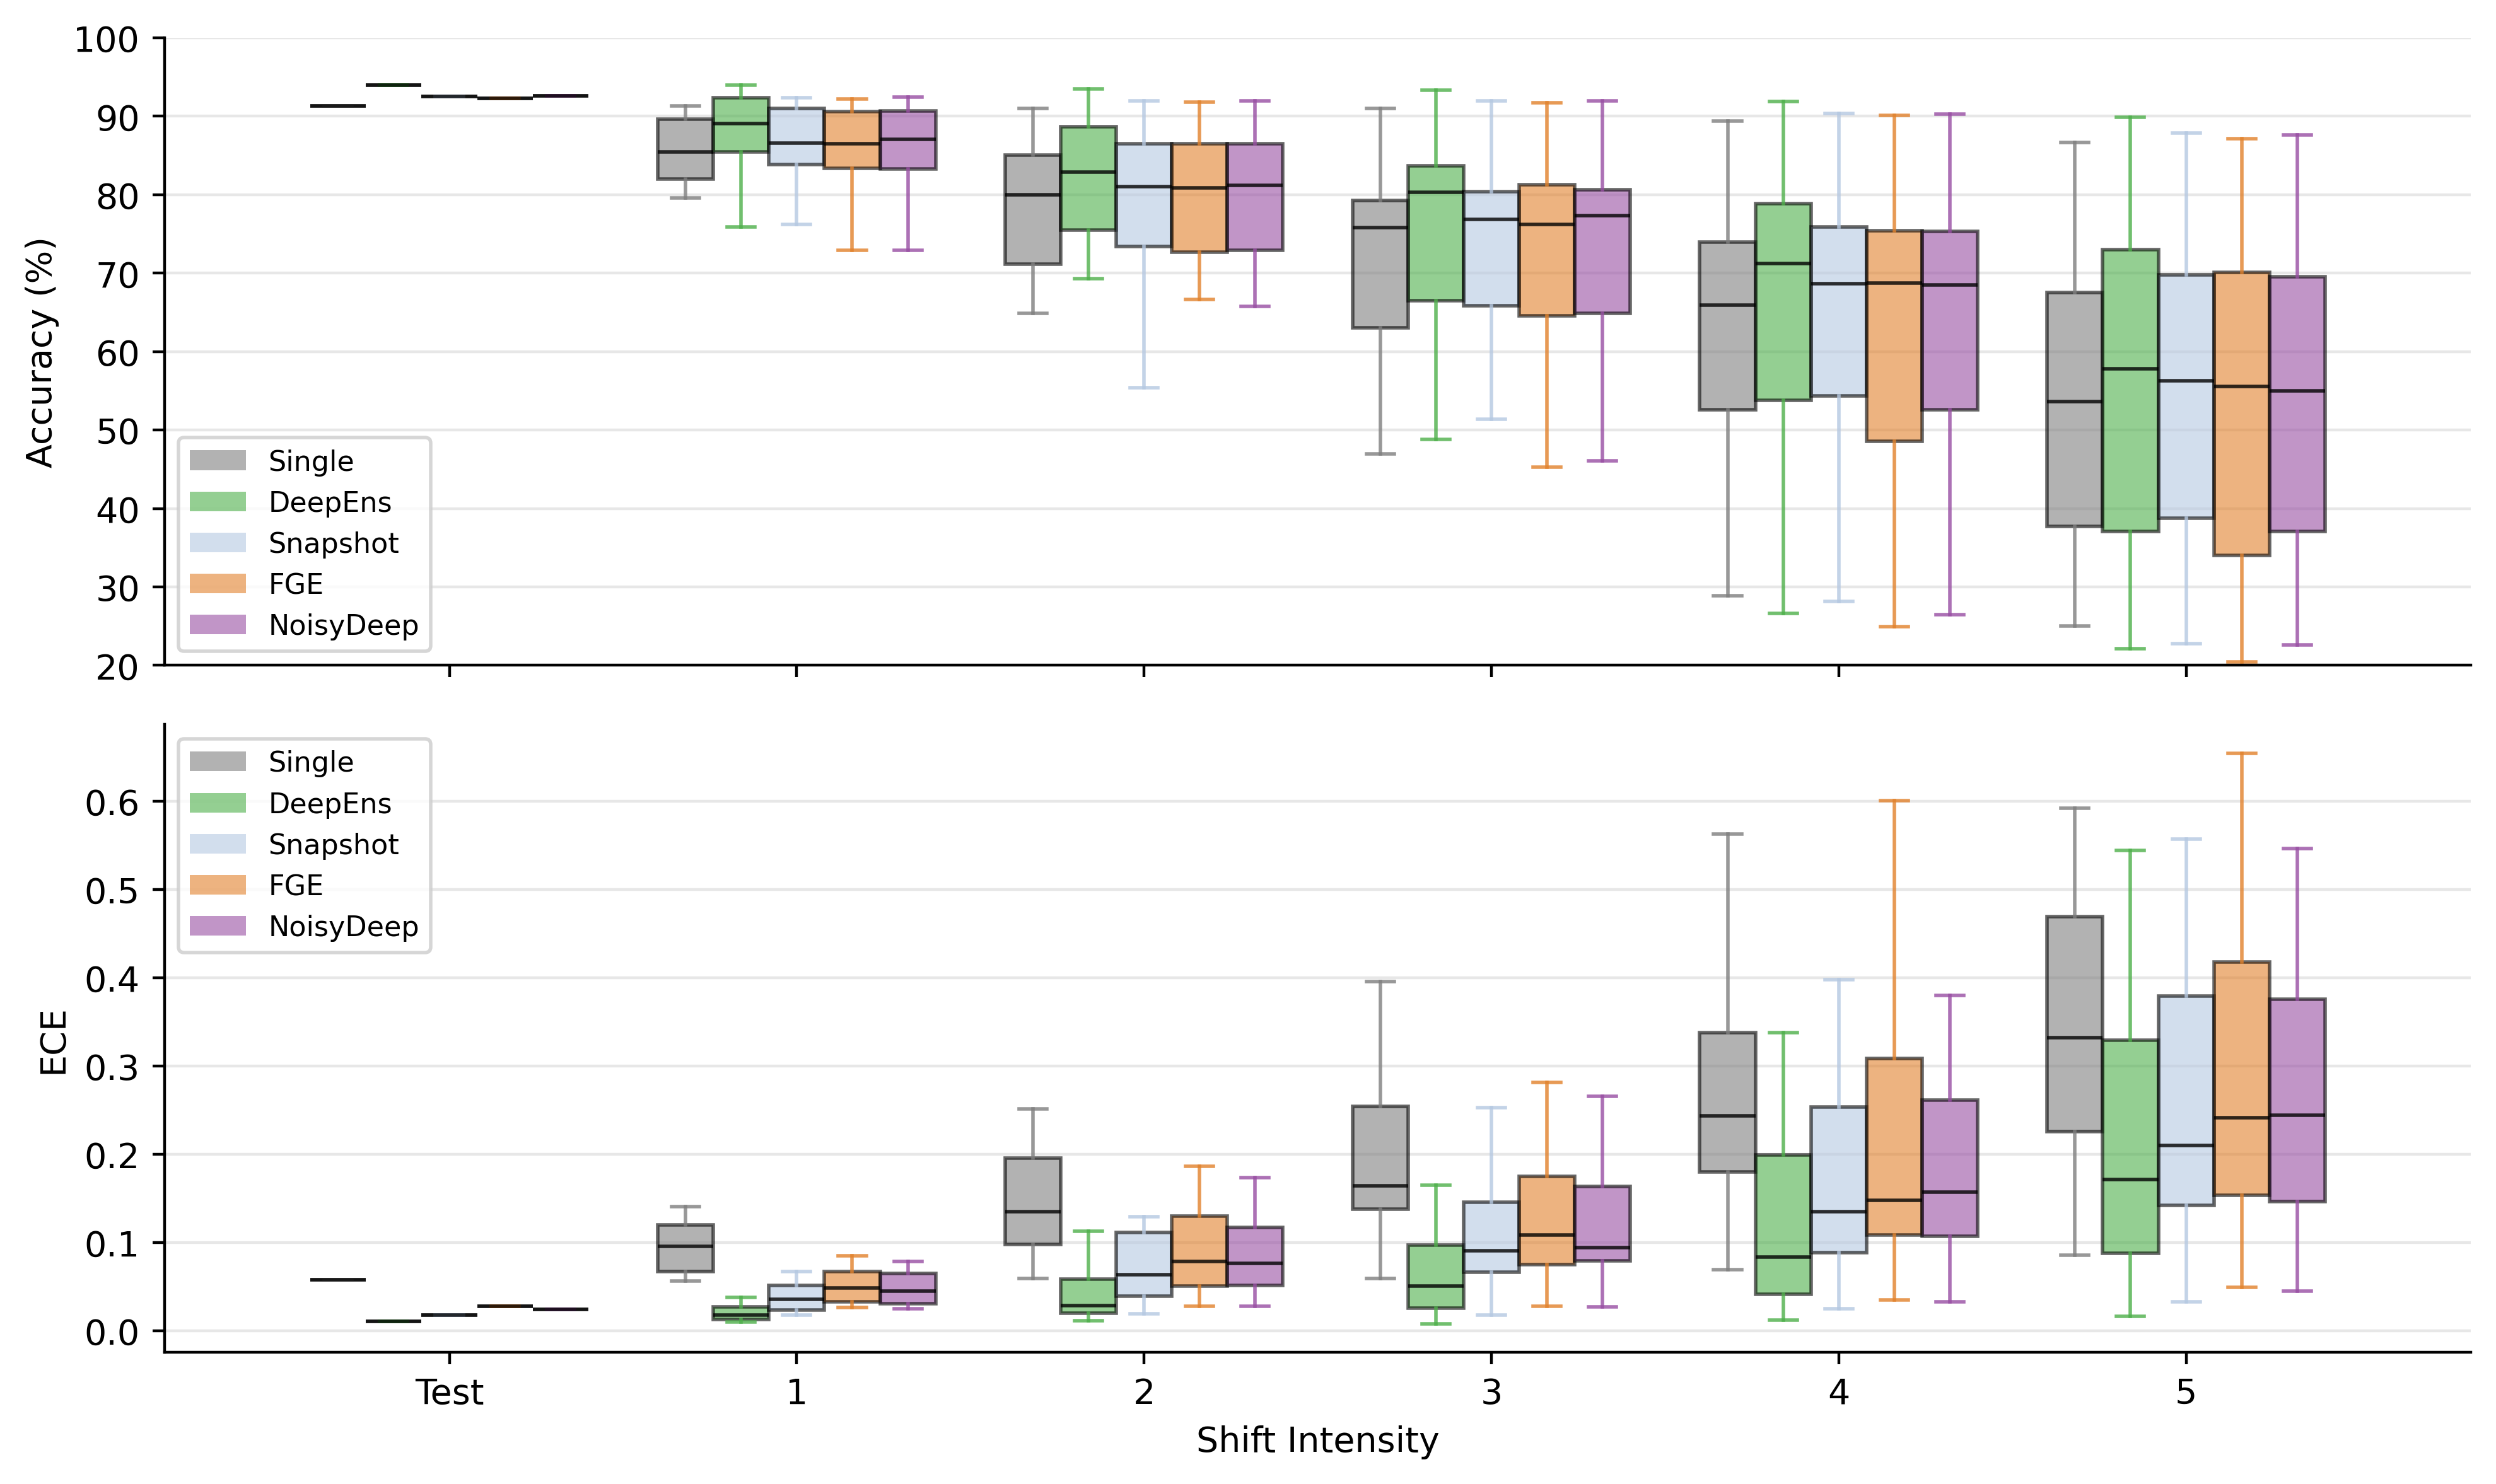
\includegraphics[width=1\linewidth]{figures/cifar10c.png}
    \caption{Figure Caption}
  \label{fig:result_figure}
\end{figure}


Fig. \ref{fig:result_figure} presents classification accuracy....



\chapter{Conclusion and Future Work}

\section{Summary of Contributions}

This thesis investigated.....
\section{Limitations}

Despite the contributions of this work....

\section{Future Work}

The current study is limited to....


%----------------------------------------------------------------------
% END MATERIAL
% Bibliography, Appendices, Index, etc.
%----------------------------------------------------------------------

% Bibliography

% The following statement selects the style to use for references.  
% It controls the sort order of the entries in the bibliography and also the formatting for the in-text labels.
\bibliographystyle{plain}
% This specifies the location of the file containing the bibliographic information.  
% It assumes you're using BibTeX to manage your references (if not, why not?).
\cleardoublepage % This is needed if the "book" document class is used, to place the anchor in the correct page, because the bibliography will start on its own page.
% Use \clearpage instead if the document class uses the "oneside" argument
\phantomsection  % With hyperref package, enables hyperlinking from the table of contents to bibliography             
% The following statement causes the title "References" to be used for the bibliography section:
\renewcommand*{\bibname}{REFERENCES}

% Add the References to the Table of Contents
\addcontentsline{toc}{chapter}{\textbf{REFERENCES}}

\bibliography{references}
% Tip: You can create multiple .bib files to organize your references. 
% Just list them all in the \bibliogaphy command, separated by commas (no spaces).

% The following statement causes the specified references to be added to the bibliography even if they were not cited in the text. 
% The asterisk is a wildcard that causes all entries in the bibliographic database to be included (optional).
\nocite{*}
%----------------------------------------------------------------------

% GLOSSARIES (Lists of definitions, abbreviations, symbols, etc. provided by the glossaries-extra package)
% -----------------------------
\cleardoublepage
\phantomsection		% allows hyperref to link to the correct page

%----------------------------------------------------------------------
\end{document} % end of logical document
